\documentclass[bachelor, och, coursework]{shiza}
% параметр - тип обучения - одно из значений:
%    spec     - специальность
%    bachelor - бакалавриат (по умолчанию)
%    master   - магистратура
% параметр - форма обучения - одно из значений:
%    och   - очное (по умолчанию)
%    zaoch - заочное
% параметр - тип работы - одно из значений:
%    referat    - реферат
%    coursework - курсовая работа (по умолчанию)
%    diploma    - дипломная работа
%    pract      - отчет по практике
% параметр - включение шрифта
%    times    - включение шрифта Times New Roman (если установлен)
%               по умолчанию выключен
\usepackage{subfigure}
\usepackage{tikz,pgfplots}
\pgfplotsset{compat=1.5}
\usepackage{float}

%\usepackage{titlesec}
\setcounter{secnumdepth}{4}
%\titleformat{\paragraph}
%{\normalfont\normalsize}{\theparagraph}{1em}{}
%\titlespacing*{\paragraph}
%{35.5pt}{3.25ex plus 1ex minus .2ex}{1.5ex plus .2ex}

\titleformat{\paragraph}[block]
{\hspace{1.25cm}\normalfont}
{\theparagraph}{1ex}{}
\titlespacing{\paragraph}
{0cm}{2ex plus 1ex minus .2ex}{.4ex plus.2ex}

% --------------------------------------------------------------------------%


\usepackage[T2A]{fontenc}
\usepackage[utf8]{inputenc}
\usepackage{graphicx}
\graphicspath{ {./images/} }
\usepackage{tempora}

\usepackage[sort,compress]{cite}
\usepackage{amsmath}
\usepackage{amssymb}
\usepackage{amsthm}
\usepackage{fancyvrb}
\usepackage{listings}
\usepackage{listingsutf8}
\usepackage{longtable}
\usepackage{array}
\usepackage[english,russian]{babel}

%\usepackage[colorlinks=true]{hyperref}
\usepackage{url}

\usepackage{underscore}
\usepackage{setspace}
\usepackage{indentfirst} 
\usepackage{mathtools}
\usepackage{amsfonts}
\usepackage{enumitem}
\usepackage{tikz}
\usepackage{minted}
\newcommand{\eqdef}{\stackrel {\rm def}{=}}
\newcommand{\specialcell}[2][c]{%
\begin{tabular}[#1]{@{}c@{}}#2\end{tabular}}

\renewcommand\theFancyVerbLine{\small\arabic{FancyVerbLine}}

\newtheorem{lem}{Лемма}

\begin{document}

% Кафедра (в родительном падеже)
\chair{теоретических основ компьютерной безопасности и криптографии}

% Тема работы
\title{Обучение с подкреплением}

% Курс
\course{3}

% Группа
\group{331}

% Факультет (в родительном падеже) (по умолчанию "факультета КНиИТ")
\department{факультета КНиИТ}

% Специальность/направление код - наименование
%\napravlenie{09.03.04 "--- Программная инженерия}
%\napravlenie{010500 "--- Математическое обеспечение и администрирование информационных систем}
%\napravlenie{230100 "--- Информатика и вычислительная техника}
%\napravlenie{231000 "--- Программная инженерия}
\napravlenie{100501 "--- Компьютерная безопасность}

% Для студентки. Для работы студента следующая команда не нужна.
% \studenttitle{Студентки}

% Фамилия, имя, отчество в родительном падеже
\author{Окунькова Сергея Викторовича}

% Заведующий кафедрой
\chtitle{доцент, к.ф.-м.н.} % степень, звание
\chname{М.~Б.~Абросимов}

%Научный руководитель (для реферата преподаватель проверяющий работу)
\satitle{Доцент} %должность, степень, звание
\saname{И. И. Слеповичев}

% Руководитель практики от организации (только для практики,
% для остальных типов работ не используется)
%\patitle{к.ф.-м.н.}
%\paname{М.~Б.~Абросимов}

% Семестр (только для практики, для остальных
% типов работ не используется)
%\term{8}

% Наименование практики (только для практики, для остальных
% типов работ не используется)
%\practtype{преддипломная}

% Продолжительность практики (количество недель) (только для практики,
% для остальных типов работ не используется)
%\duration{4}

% Даты начала и окончания практики (только для практики, для остальных
% типов работ не используется)
%\practStart{30.04.2019}
%\practFinish{27.05.2019}

% Год выполнения отчета
\date{2022}

\maketitle

% Включение нумерации рисунков, формул и таблиц по разделам
% (по умолчанию - нумерация сквозная)
% (допускается оба вида нумерации)
% \secNumbering

%-------------------------------------------------------------------------------------------
\tableofcontents

\intro

В наше время компьютеры стали очень важной частью наше жизни. Существует огромный пласт задач, решение
которых мы уже не представляем без его использование. Большую часть из этих задач сегодня можно решить с помощью классического
программирования, однако другую часть задач решить с помощью него либо очень проблематично, либо вовсе не возможно. Эти 
задачи как правило связанны либо с искуственным интелектом, либо с нахождением закономерности в большом объеме данных.
Такие задачи решаются с помощью специальных подходов, которые в совокупности называются машинным обучением. Основное
приемущество данного подхода заключается в более эффективном методе построения вычислительных систем – обучаемых систем,
вместо систем, программируемых. 

На сегодняшний день направление машинное обучение занимает одну из ведущих позиций в IT, поэтому оно также является одним
из самых развивающихся, чем и обусловлено появление каждый год новых алгоритмов и задачи. Если раньше с помощью машинного
обучения можно было решать только просты задачи с поиском закономерностей в данных, сейчас существует множество областей,
в которых алгоритмы машинного обучения превосходят человека. Вот несколько примеров задач, которые решают с помощью
машинного обучения: распознование и классификация объектов на изображении, классификация текста, распознование речи, 
выдача рекомендаций, основанных на наших предпочтениях, перевод текста с картинки, принятие решений по выдаче кредитов,
прогнозирование цен на квартиры, технику и другие товары и т. д.. Данная работа посвящена рассмотрению концепции обучения
с подкреплением, задачам, решающимся с помощью данного вида обучения, и алгоритмы, построенные для решения этих задач.

В отличие от классического машинного обучения, в обучении с подкреплением изначально нет никакой выборки для обучения модели.
Вместо этого, обучение проводится "методом проб и ошибок": агент сам собирает данные о среде, в которой находится, и на 
основе этих данных и своих действий пытается наиболее эффективно выполнить свою цель, которую он определяет так же сам за
счет системы наказаний и пощрений, заданной ему в самом начале.

\section{Теоритическая часть}

\subsection{Понятия искусственного интелекта, машинного и глубокого обучения}

\textbf{Искусственный интелект (ИИ, AI, Artificial intelligence)} - это наука, описывающая создание машины или программы,
способной имитировать человеческое поведение для выполнения определенной задачи и обучаться за счет полученной в результате
работы информации.

Другими словами ИИ можно описать, как технологию, которая способна мыслить как человек и выполнять функции человека с большей
точностью. На практике же достаточно сложно создать идеальную модель ИИ, способного грамотно выполнять заданные ей функции. 
Поэтому для решения большинства задач в этой сфере используют машинное обучение.

\textbf{Машинное обучение (Machine learning, ML)} - это метод анализа данных, который автоматизирует построение аналитической 
модели.[1] Данная область ИИ воплощает в себе идею того, что машина способна обрабатывать полученные данные, анализировать их 
и на основе анализа обучаться с минимальным вмешательством человека.

Однако данная область ИИ всеже требует помощи в самом процессе обучения со стороны человека, а именно загрузку корректных данных,
рассматривающих все возможные случаи, на которых машина будет обучаться. Иначе говоря, несмотря на то, что данная система обучения
машины позволяет решить огромное количество задач, она не способна сама генерировать эти задачи.

\textbf{Глубокое обучение (глубинное обучение, Deep learning, DL)} - это тип машинного обучения, который обучает компьютер выполнять 
задачи человека.[1]

Данная система обучения вместо того, чтобы ждать тесты от человека, для дальнейшей их обработки по формулам, заданным изначально,
сама устанавливает начальные параметры и учит машину обучаться самостоятельно.

Таким образом, если представить AI, ML и DL в виде трех множеств, то мы получим картину, изображенную на рисунке 1:

\begin{equation}
    DL \subset ML \subset AI. 
\end{equation}

\begin{figure}[H]
    \centering
    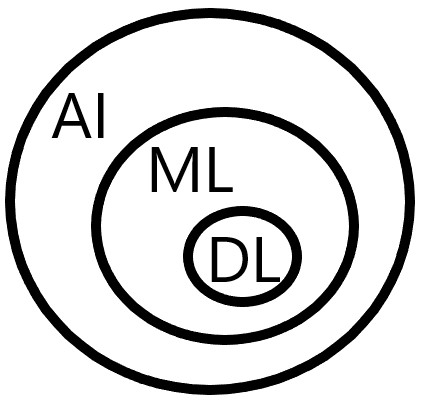
\includegraphics[width=0.35\textwidth]{pic/2}
    \caption{Представление AI, ML и DL в виде множеств}
    \label{fig:img1}
\end{figure}

\subsection{Структура искусственной нейронной сети}

Для решение задач в сфере машинного и глубокого обучения часто используют искусственные нейронные сети.

\textbf{Искусственные нейронные сети (ИНС, artificial neural networks, ANN)} - математическая модель и ее програмное воплощение, созданное
на основе модели биологических нейронных сетей (сетей нервных клеток организма).

ANN состоит из искусственных нейронов (ИН, artificial neuron, AN), являющихся програмной реализацией нейронов живых организмов и представляющих
из себя нелинейную функцию, называемую передаточной функцией, от массива входных данных ([$x_1, x_2, ..., x_n$]). Основная функция ИН - принятие 
входного сигнала с последующей его обработкой и передачей результата на другие нейроны.

Из всего выше описанного очевидно, что некоторые AN связаны между собой. Как и в биологии данную связь называют синоптической связью.

\textbf{Синапсом} в искусственных нейронных сетях называют связь между нейронами. По нему передаются выходные связи с одного нейрона на 
другой. У любого синапса имеется такой параметр, как весовой коэффициент $w_i$, который показывает текущее состояние нейрона, а более сложные 
синапсы также могут иметь память. Состояние нейрона в определенный момент времени вычисляется как взвешенная сумма его входов:

\begin{equation}
    s = \sum\limits_{i=1}^nx_iw_i,
\end{equation}
где n - число входов нейрона, $x_i$ - i-й входной сигнал, $w_i$ - вес i-го синапса.

В большинстве случаях связь между нейронами представляют в виде матрице W, которую соответственно называют матрицей веса.

Помимо синапсов важную роль в связи нейронов между собой играют аксоны. \textbf{Аксон} - это выходная связь нейрона, с помощью которой выходной 
сигнал нейрона поступает на синопсы других нейронов. Его значение будет равно:

\begin{equation}
    Y = f(s),
\end{equation}
где $s$ - это состояние нейрона в данный момент, а $f$ - это передаточная функция, в качестве которой чаще всего используются сигмоид, линейный порог,
гиперболический тангенс или жесткую пороговую функцию. Данная функция одинакова для нейронов одного слоя, но для нейронов разных слоев она могут
выбираться разные функции.

Проанализировав все выше описанное можно представить, как в общем выглядит нейрон:

\begin{figure}[H]
    \centering
    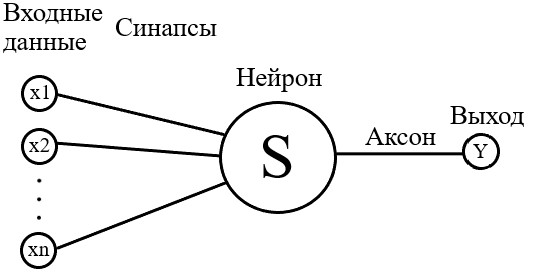
\includegraphics[width=0.5\textwidth]{pic/3}
    \caption{Общий вид искусственного нейрона}
    \label{fig:img1}
\end{figure}

Уже на данном этапе достаточно информации, чтобы сделать вывод о том, как схематически можно изобразить искуственную нейронную сеть. Пример такого
изображения можно увидеть на рисунке 3.

\begin{figure}[H]
    \centering
    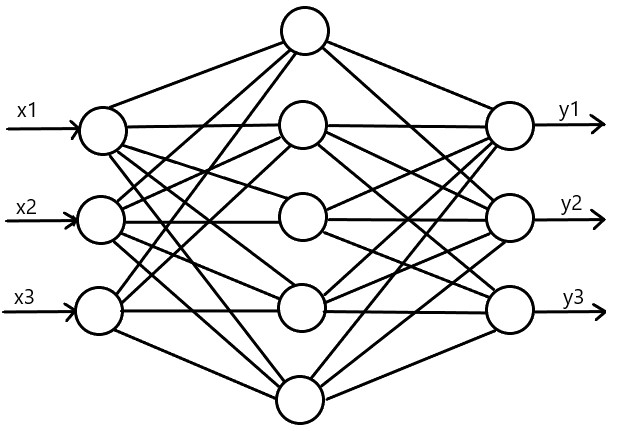
\includegraphics[width=0.55\textwidth]{pic/4}
    \caption{Пример искусственной нейронной сети}
    \label{fig:img1}
\end{figure}

\subsection{Обучение искусственной нейронной сети}

Как говорилось выше, для решения задачи не достаточно просто написать модель нейросети, ее еще нужно и обучить. Под процессом обучения понимается выбор
таких параметров, при которых нейросеть решает поставленную задачу с большей эффективностью. Схема обучения изображена на рисунке 5. Математически его 
можно описать следующим образом. В процессе работа нейросеть, как было выясненно выше, формирует выходной сигнал $Y = G(X)$, являющийся реализацией какой-то
функции. И пусть ответом на поставленную задачу будет функция $Y = F(X)$, заданная с помощью параметра входных-выходных данных так, что

\begin{equation}
    Y^k = F(X^k),
\end{equation}
где $k = 1, ..., N$ - это номер элемента заданной выборки данных.

Обучением же будет состоять из генерации функции $G(X)$, близкой к $F(X)$. Оно будет состоять из множества итераций, на каждой из которых функция $G(X)$ будет
все ближе и ближе к функции $F(X)$, а для определения степени их близости друг к другу используют некоторую функцию $D_F(G)$, которую называют функцией ошибок или
целевой функцией. Каждую такую итерацию называют эпохой. Таким образом обучение ИНС будет проходить до того момента, пока функция $D_F(G)$ не примет минимальное свое значение.

\begin{figure}[H]
    \centering
    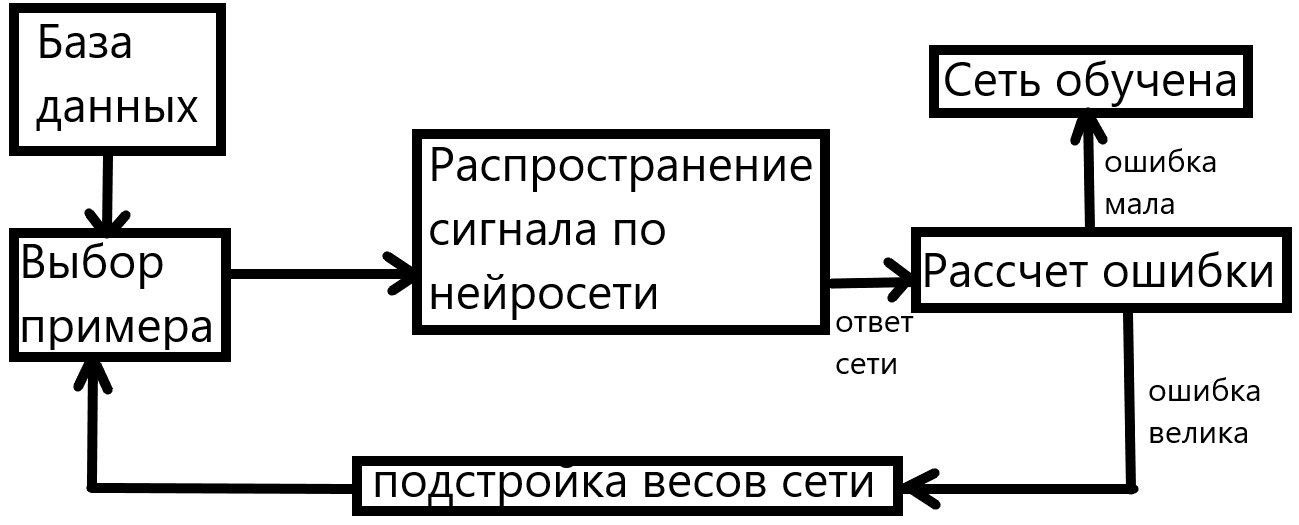
\includegraphics[width=0.85\textwidth]{pic/5}
    \caption{Процесс обучения нейронной сети}
    \label{fig:img1}
\end{figure}

Выбираемые параметры делятся на два вида:

\begin{enumerate}
    \item Гиперпараметры - это такие параметры, которые настраивает сам человек до запуска самого процесса обучение (например количество эпох обучения);
    \item Веса модели - это те параметры, которые настраиваются самой моделью при обучении. Они показывают значимость каждого нейрона в функции $G(X)$.
\end{enumerate}

Одним из важнейших гиперпараметров практически любой модели является скорость обучения (learning rate). С помощью него задается скорость схождения функции
$G(X)$ к функции $F(X)$ на каждой итерации.

Существует три основные стратегии обучения, используемые для решения разного вида задач:

- с учитетелм или по другому контролируемое обучение (Supervised Learning)- нейросети на вход подаются данные и она обучается путем обработки этих данных;

- без учителя или по другому неконтролируемое обучение (Unsupervised Learning) - нейросеть обучается в соответствии с некоторым правилом, при этом данные для обучения не требуются;

- обучение с подкреплением (Reinforcement learning) - имеет сходство с обучением с учитетелм, только в роли учителя выступает настоящая или виртуальная среда.

\subsection{Обучение с подкреплением (Reinforcement learning)}

Данный вид обучения имеет сходство с человеческим обучением: человек хочет чему-то научится, для этого он делает какие-то действия, у которых есть некоторые
последствия (как положительные, так и отрицательные), и относительно этих последствий корректирует свои действия в дальнейшем. Другими словами модель, обучаемая
с помощью RL, изначально не имеет никаких сведений о среде, в которой находится, но имеет возможность выполнять определенные действия в ней, чтобы лучше
понимать эту среду, за счет чего и обучается.

Таким образом фокус обучения с подкреплением делается на регламентированные процессы обучения, при которых алгоритм машинного обучения снабжен набором действий, параметров и конечных значений.[11]

\textbf{Агентом} называют некоторую сущность, которая выполняет определенные действия в среде. Модель же в данном случае по состоянию среды и агента в ней
в данный момент прогнозирует действие, которое должен совершить агент для того, чтобы приблизится к выполнению задачи максимально эффективно. Для достижения
этой эффективности инжинером изначально задается система штрафов и пощрений, т. е. при достижении определенного состояния агента и среды модель либо добавляются очки
(например прохождение агентом некоторого расстояния), либо вычитаются очки (например смерть агента). Иными словами у обучения с подкреплением построенно на двух
основных принципах, совокупность которых была названа выше эффективностью:

\begin{enumerate}
    \item Минимизация ошибок (например уменьшение количества столкновений с другими машинами и т. д.);
    \item Максимизация выгоды, заданной заранее (например максимально быстрое время прохождения заданной дистанции, минимальное количество расходуемых ресурсов и т. д.).
\end{enumerate}

Определим терминологию:

\begin{itemize}
    \item $S_t$ - состояние среды (state) на шаге t;
    \item $a_t$ - действие агента (action) на шаге t;
    \item $r_t$ - награда (reward) на шаге t;
    \item $\pi(a_t|s_t)$ - policy, стратегия поведения агента, условная вероятность;
    \item $a_t\sim\pi(\cdot|s_t)$ - action рассматриваем как случайную величину из распределения $\pi$,
    Мы могли бы рассматривать policy как функцию $\pi:States\to Actions$, но мы хотим сделать действия агента стохастическими, что способствует exploration.
    Т.е. мы с некоторой вероятностью делаем не совсем те действия, которые выбирает агент.
    \item $\tau$ - траектория, пройденная агентом, последовательность $(s_1, s_2, ..., s_n) $;
    \item $V$ (value) или $E$ (estimate) - ожидаемая итоговая (награда) со скидкой, в отличии от мгновенной награды $R$, является функцией политики $E^\pi(s)$ и
    определяется, как ожидаемая итоговая награда Политики в текущем состоянии $s$. (Встречается в литературе два варианта Value - значение, Estimate - оценка,
    что в контексте предпочтительней использовать $E$ - оценка);
    \item $R_i$ - общая награда за $i$ эпизод;
    \item Q-value (Q) - оценка $Q$ аналогична оценке $V$, за исключением того, что она принимает дополнительный параметр $a_t$. $Q^\pi(s_t, a_t)$ является итоговой
    оценкой политики $\pi$ от состояния $s_t$ и действия $a_t$. Рассчитывается с помощью уравнения Беллмана:
    \begin{equation}
        Q(s, a) = r(s, a) + \gamma max(Q(s', a)). [25]
    \end{equation}
\end{itemize}

Оно означает, что максимально возможное вознаграждение $(Q)$ агента в состоянии $s$ равно сумме моментального вознаграждения $r$ за его шаг $а$ и максимально возможноного вознаграждения агента
из состояния $s'$ помноженное на коэффициент понижения $\gamma$.

\begin{figure}[H]
    \centering
    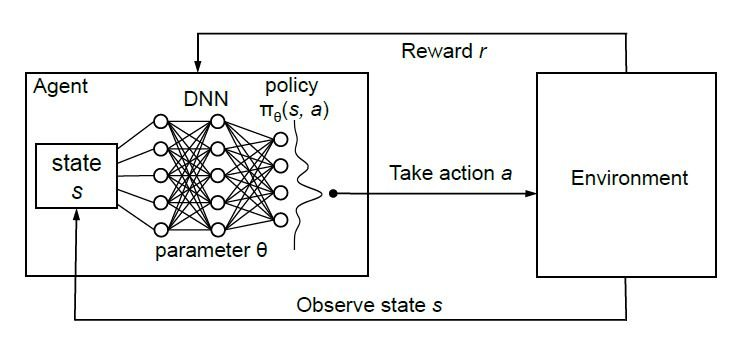
\includegraphics[width=0.85\textwidth]{pic/7}
    \caption{Взаимосвязь агента и среды[25]}
    \label{fig:img1}
\end{figure}

Задача агента — максимизировать expected return:

\begin{equation}
    J(\pi)=E_{\tau\sim\pi}[R(\tau)]=E_{\tau\sim\pi} \left[\sum_{t=0}^n r_t\right]. [25]
\end{equation}

Таким образом математически задачу RL можно сформулировать как поиск такой оптимальной стратегии $\pi^*$, что $\pi^* = arg \mathop {max} _ \pi J(\pi)$[25].

Таким образом можно сделать вывод, что обучение с подкреплением полностью завязано на взаимном воздействии агента и среды вне зависимости от алгоритма.
О такой системе говорят, что она имеет обратную связь, поэтому ее нужно рассматривать как единое целое, из-за чего линия разделения между средой и агентом
в этой системе достаточно условна. Эта взаимосвязь схематично показана на рисунке 5. Эта взаимосвязь рассматривют как последовательность пар state и
reward, переходами в которые являются actions агента:

\begin{equation}
    (s_0) \stackrel{a_0}{\rightarrow} (s_1, r_1) \stackrel{a_1}{\rightarrow} ... \stackrel{a_{n-1}}{\rightarrow} (s_n, r_n). [25]
\end{equation}

\subsection{Оценка качества обученной модели}
После окончания процесса обучения необходимо проверить насколько хорошо модель обучилась. Для этого используют метрики качества обучений. Существует множество хороших метрик,
которые используются для разных задач, поэтому очень важно правильно выбрать метрику для выбранной задачи.

В задачах Reinforcement learning лучшими метриками являются награда за эпоху или средняя награда за несколько эпох:
\begin{equation}
    \frac{1}{n}\sum^n_{i = 0} R_i.
\end{equation}

\subsection{Сверточная нейронная сеть}

Для некоторых алгоритмов обучения с подкреплением используют сверточные нейронные сети, поэтому их также стоит рассмотреть для лучшего понимания темы данной работы.

Наилучшие результаты в задачах распознования объектов на изображениях показала \textbf{сверточная нейронная сеть (Convolutional Neural Network, CNN, СНС)}, 
которую называют логическим продолжением идей когнитрона и некогнитрона. Главной причиной успеха данной архитектуры является учет двумерной тополгии изображения.
СНН работает по принципу маштабирования (свертки) изображения.

\textbf{Свертка} - это операция над исходной матрицей $A$ и матрицей свертки $B$, размерностью  ($n_x * n_y$) и ($m_x * m_y$) соответственно, результатом которой является матрица $C = A * B$,
размер которой ($n_x - m_x + 1 * n_y - m_y + 1$), а элементы расчитываются по формуле:
\begin{equation}
    C_{i,j} = \sum\limits_{u=0}^{m_x-1}\sum\limits_{v=0}^{m_y-1}A_{i+u,j+v}B_{u,v}. [25]
\end{equation}

\begin{figure}[H]
    \centering
    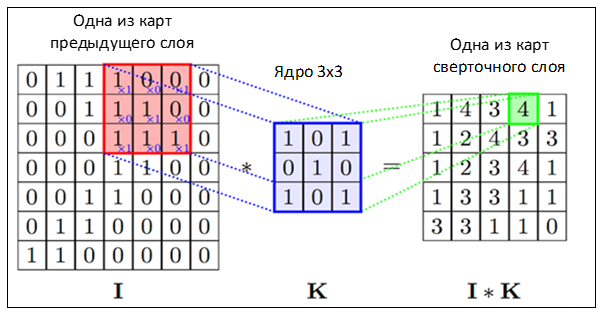
\includegraphics[width=0.85\textwidth]{pic/6}
    \caption{Свертка[6]}
    \label{fig:img1}
\end{figure}

Архитектура данного типа ИНС строится на чередовании слоев свертки и подвыборки, которые состоят из карт признаков. Они в свою очередь отвечают за поиск определенных
признаков. К примеру одна карта ищет предметы красного цвета, вторая - синего.

\subsection{Задачи, решаемые с помощью обучения с подкреплением}
Обучение с подкреплением применяется там, где принятое решение может иметь последствия не только сразу после его принятия,
но и спустя некоторый промежуток времени. Поэтому алгоритмам данного вида обучения иногда приходится ждать, чтобы
увидеть последствия своих решений. Обычно даже человеку в таких задачах сложно понять, какой порядок действий приводит к
какому результату.

К таким задачам относятся:
\begin{enumerate}
    \item Создание продвинутого ИИ для игр. Сейчас большинство ИИ в играх создаются на основе математических автоматов с множеством состояний
    и переходов. Однако этот подход является не самым совершенным, и поэтому качество такого ИИ оставляет желать лучшего. Подход же с нейросетью,
    обученной с помощью RL, является более совершенным. Так такие ИИ могут спокойно обыгрывать чемпионов мира по шахматам или представлять реальную
    угрозу даже самым умелым игрокам. Ярким примером является OpenAI Five. [21]
    \item Обучение модели для автономного вождения. Изначально моделируется несколько различных сред для машины, которая в данном случае является агентом,
    а затем в них по очереди помещается сам агент для обучения на всех возможных ситуациях. Так сначала модель обучется на пустой дороге, чтобы модель понимало,
    что агент должен ехать только по ней по ней, затем агента запускают в среду с пешеходами и знаками дорожного движения, чтобы научить модель соблюдать ПДД,
    а после его начинают запускать в среды, которые представляют из себя различные специфичные ситуации: зимние дороги, непогоду, ремонтные работы, поломанные
    дороги и т.д. Ярким примером использования алгоритмов RL в данной сфере являются машины компании Tesla. [12]
    \item Обучение роботов в робототехнике. Схоже с предыдущим пунктом, меняются лишь цели обучения, возможности действий агента, условия самих сред и их количество
    в зависимости от самой задачи. [12]
    \item Чат боты, основанные на нейронных сетях. Для данной задачи существует несколько подходов. Первый из них представляет из себя создание огромного ансамбля
    NLP (Natural Language Processing) моделей, работающих как паралельно, так и последовательно. Второй же завязан на одной модели, обученной с подкреплением. В
    этом случае средой выступают диалоги с обычным пользователем, а агентом сам чат бот. [22]
    \item Рекомендательные системы. Данный класс задач тоже можно решать с помощью RL. Тогда выдача рекомендации того или иного предложения будет являтся действием в среде,
    а средой будет выступать совокупность того место, где будет появлятся рекомендация и людей, находящихся в данной среде. Этот подход в преспективе является лучше
    классического двухуровневого подхода к данной задаче, однако проигрывает ему в скорости обучения, потому что в двухуровневом подходе обучение происходит
    перед испльзованием модели, за счет чего мы получаем неплохое качество рекомендаций уже после добавления такой функции, а RL моделью обучается при 
    взаимодействие с ней пользователей. [23]
\end{enumerate}

\subsection{Алгоритмы RL}
\subsubsection{Наивные подходы}
Самый постой подход к данному классу очень просто и не предполагает использование ИНС. Его реализация представляет собой использование динамического программирования и
состоит из двух шагов:
\begin{enumerate}
    \item Перебрать все возможные стратегии.
    \item Найти самую оптимальную стратегию, дающую наибольшую награду.
\end{enumerate}
Главная проблема такого подхода - это количество стратегий, которые надо обработать. Их колличество может быть не просто очень велико, а бесконечно. Вторая проблема
заключается в плохом обобщении такой системы. Использование ИНС хорошо решает эти проблемы, не рассматривая все стратегии, а выбирая, основываясь на своем опыте
предыдущем опыте, оптимальную.

Данную задачу можно также попробовать решить стандартыми алгоритмами, обучая их с подкреплением, однако такое решение не принесет нужный результат вне зависимости от сложности модели.
Так происходит по одной простой причине, которая заключается в дизбалансе классов, вызванный случайными действиями агента в ситуациях, в которых он не знает как действовать,
из-за чего некоторые действия могут вовсе не воиспроводится. Более простыми словами полезные сигналы теряются на фоне шума, который обусловлен редкими наградами. Поэтому для
задач RL используют специальные алгоритмы. Список таких алгоритмов можно увидеть на рисунке 7.

\begin{figure}[H]
    \centering
    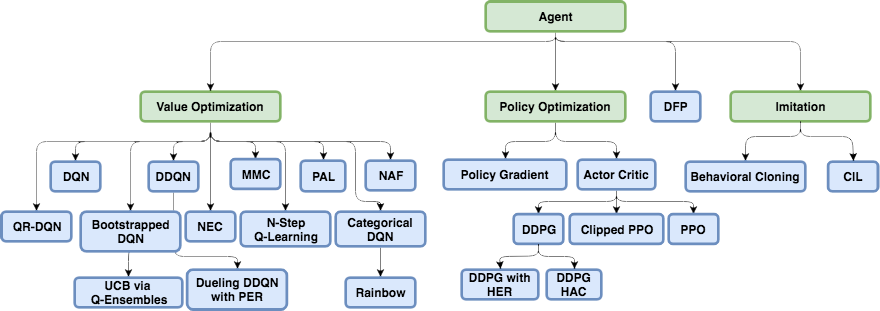
\includegraphics[width=0.85\textwidth]{pic/9}
    \caption{Алгоритмы RL[19]}
    \label{fig:img1}
\end{figure}

\subsubsection{Q-learning}
Раньше, когда НС не существовало, а мощностей компьютера не хватало для высоконагруженных вычислений, уже существовал RL. Он выглядил как простая, но очень оригинальная идея:
делать случайные действия, а потом для каждой ячейки в таблице и каждого направления движения, посчитаем по формуле уравнения Беллмана (6) насколько хороша эта ячейка и выбранное направлени. Чем
выше это число, тем с большей вероятностью этот путь ведет к большей выгоде. Само такое число получило название Q (от слова quality — качество выбора, очевидно), а метод —
Q-learning.
\begin{figure}[H]
    \centering
    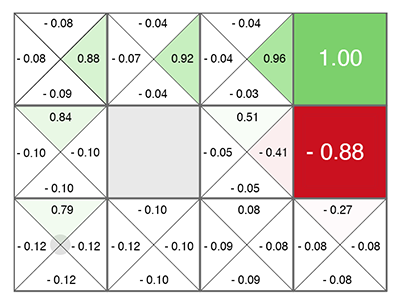
\includegraphics[width=0.65\textwidth]{pic/8}
    \caption{Пример табличного RL[19]}
    \label{fig:img1}
\end{figure}
Чтобы побороть проблему обычных ИНС, описанную выше ученые вернулись к классическому табличному Reinforcement Learning, но вместо ручного подсчета значений таблицы в качестве
целевой функции стали использовать НС. На основе этого подхода и строятся алгоритмы RL сегодня и, он же является отличием от обычного обучения нейросетей. Классический же
алгоритм, в основе которого лежит только заполнение таблицы получил название DQN (Deep Q-learning Network)[20].

В DQN на вход нейросети подается текущая ситуация (state), а на выходе нейросеть предсказывает число Q. А так как на выходе сети перечислены сразу все возможные действия
(каждый со своим предсказанным Q), то получается что нейросеть в DQN реализует классическую функцию Q(s,a) из Q-learning. Следовательно для получения самого оптимального
действия в заданной ситуации нужно использовать argmax, для который вернет индекс действия с максимальным Q. Такая политика будет называться детерменистской. Но более
оптимальной будет стохастическая политика. При ней выбирается случайное действие з доступных, но пропорционально их Q-значениям (т.е. действия с высоким Q будут выбираться
чаще, чем с низким). Такая политика является более оптимальной, так как она выбирает действия, которые в данный момент могут не нести особого смысла в данный момент, но могут
в дальнейшем привести к действиям с большей наградой и меньшим штрафам.

Гланый минус такого алгоритма, что он работает только с агентом, который может совершать небольшое колличество детерминированных действий (при их высоком количестве метод просто не сходится).
Чтобы решить данную проблему были придуманны другие алгоритмы, оптимизатором для которых стал модифицированный алгоритм градиентного спуска, получивший название Policy Gradient.

\subsubsection{Policy Gradient}
Идея алгоритма очень проста: подавать на вход НС текущее состояние, на выходе сразу предсказывать действия $\pi_\theta(a_t|s_t)$, а затем сравнивать полученную награду за действие
со средней наградой. Таким образом по динамике $R(\tau) = \sum_{t=0}^T r_t$ становится возможно вычислять вектор градиент. Эта модификация позволяет свести задачу обучения RL сети к
обычной задачи классификации, следовательно в качестве функции потерь можно использовать модифицированную версию кросс-энтропии:
\begin{equation}
    loss = -log(\pi_\theta(a_t|s_t))R(tau). [25]
\end{equation}
За счет этого происходит уменьшение шума, который не давал корректно обучать классические модели НС для класса задач RL.

Приемуществом данного метода является возможность обучать модель с большим количеством действий, а также гибкая система пощрений и наказаний. К минусам же можно отнести
то, что пересчет весов модели происходит только в конце эпохи, а не с каждым шагом агента.[15]
\subsubsection{Actor-critic}
Следующая модификация, которая была добавлена в алгоритмы RL, это добавление явного учителя, который представляет из себя новую модель, которая будет оценивать действия
агента. Такую модель называют критиком, а агента - актером.

Актерская модель практически ничем не отличается от стандартной архитектуры агента. На вход так же подается состояние среды в данный момент и на выход выдается действия
или вектор вероятностей уместности действий в данной ситуации.

Критическая модель получает на вход так же получает состояние и действие, предсказанное первой моделью, а на выход ввыводет значение значению $Q$, которое будет
являться функцией от входных параметров $Q(s, a)$.Таким образом за счет оценки критика обучается актер на основе Police Gradient, а критик будет учится обычным
путем, согласно с реальным прохождением эпизода.

Примером алгоритма использующего классическую реализацию Actor-critic является DDPG. Более продвинутые модели способны сравнивать новую политику с предыдущей
и на основе этого корректировать свои веса. В этом случае для рассчета градиента используется не просто функция $Q(s,a)$, а $A(s,a) = Q(s,a) - V(s)$.[25] В данном случае
функция $A(s, a)$ как раз и показывает насколько после предпринятых действий станет лучше, чем текущая ситуация $V(s)$(в самой простой реализации $Q(s,a)$ можно
заменить на $r$ и таким образом $A = r - V(s)$). Примером таких алгоритмов являются A3C/A2C. Их главным минусом является резкое изменение весов моделей из-за чего
процесс спуска становится более стохастическим, поэтому более поздние алгоритмы, такие как Proximal Policy Optimization (PPO)[15] и Trust Region Policy Optimization (TRPO)[15]
имеют ограничению на изменение весов (что-то вроде gradient clipping в рекуррентных сетях для защиты от взрывающихся градиентов, только на другом математическом аппарате),
один из которых и используется в практической части данной работы.

\section{Практическая часть}
\subsection{Описание используемых инструментов}
В качестве языка программирования для данной работы был выбран Python 3.9.5, потому что на сегодняшний день данный язык программирования он является самым привлекательным
языком для работы с глубоким обучением, имея только одну хорошую альтернативу в лице языка R. Это связано не только с простатой работы с языком, но и с большим списком
фреймворков для ML.

Чтобы проводить эксперементы с моделью и средой была использована платформа Jupyter Notebook. С помощью этой платформы создается локальный сервер, на котором можно работать
с файлами с расширением .ipynb. Плюсом таких файлов является возможность запускать не весь код, написанный на языке Python, а лишь его части, хранящиеся в отдельных ячейках.
Это очень удобно, потому что весь код можно хранить в одном файле и запускать только необходимые в данный момент его части, за счет чего становится проще отлаживать конечную программу.

Для обработки состояния среды с помощью скриншота была выбрана библиотека OpenCV[26]. Она за счет своего широкого функционала обработки изображений любого формата часто используется
в задачах компьютерного зрения. В данный функционал входит возможность накладывать фильтры на изображение, покадрово обрабатывать видеозаписи, изменять размерность изображений и
многие другие полезные функции.

Также в качестве инструмента для создания среды, в которой будет обучаться модель была выбрана одна из лучших библиотек, созданных специально для RL, OpenAI Gym[27]. Эта
узкая направлнность библиотеки и является ее главным плюсом. С помощью нее можно эффективно определить правила, по которым существует среда (за что агент будет получать
награду, а за что штраф, как обрабатывать каждое состояние, что будет происходить, после окончание каждого эпизода, количество возможных действий агента и т.д.).

В качестве фреймворка для работы с моделью была выбрана библиотека Stable Baselines3, содержащая в себе модели RL, написанные с помощбю более широкоиспользуемой библиотеки PyTorch.
Поэтому плюсы библиотеки PyTorch[25] также сохраняются в библиотеке Stable Baselines3[24].

Для визуализации кривых обучения, представляющих из себя метрики обучения был использован очень попуярный инструмент tensorboard, созданный специально для этого. Его плюс в том,
что в отличии от популярных фреймворков визуализации matplotlib или seaborn нет необходимости писать небольшой скрипт на языке python, а достаточно лишь одной команды в терминале
для того, чтобы создать на локальном сервере доску с визуализацией результата обучения.

\subsection{Описание среды и агента}
В качестве среды, в которой будет проходить, обучения был взять один из сценариев игры DOOM, созданой компанией Id-softwer и выпущеной в 1993 году, ставшей одним из первых FPS
(шутеров от первого лица), а именно сценарий deadly_corridor.[28] Целью агента в данном сценарии является пройти до конца коридор и взять броню, избегая урона от вражеских ИИ, реализованных
с помощью классического математического автомата.

С помощью средств библиотеки OpenAI Gym были определены основные правила данной среды обучения, включая функцию награды за действие:

\begin{equation}
    r = movement\_r - \Delta damage*10 + \Delta hitcount*200 - \Delta ammo*5,
\end{equation}
где $\Delta damage$ - урон, полученный агентом за шаг, $\Delta hitcount$ - урон нанесенный агентом за шаг, $\Delta ammo$ - количество патронов, потраченных агентом на текущем
оружие, $movement\_r$ - встроенная награда среды за шаг агента, определяющаяся следующим образом: если агент идет в сторону брони, она линейно увеличивается на 1.2 иначе,
счетчик сбрасывается и по такому же принципу рассчитывается штраф, только вместо увеличения счетчика идет его уменьшение.

Код для настройки среды находится в файле environment.py.

\begin{figure}[H]
    \centering
    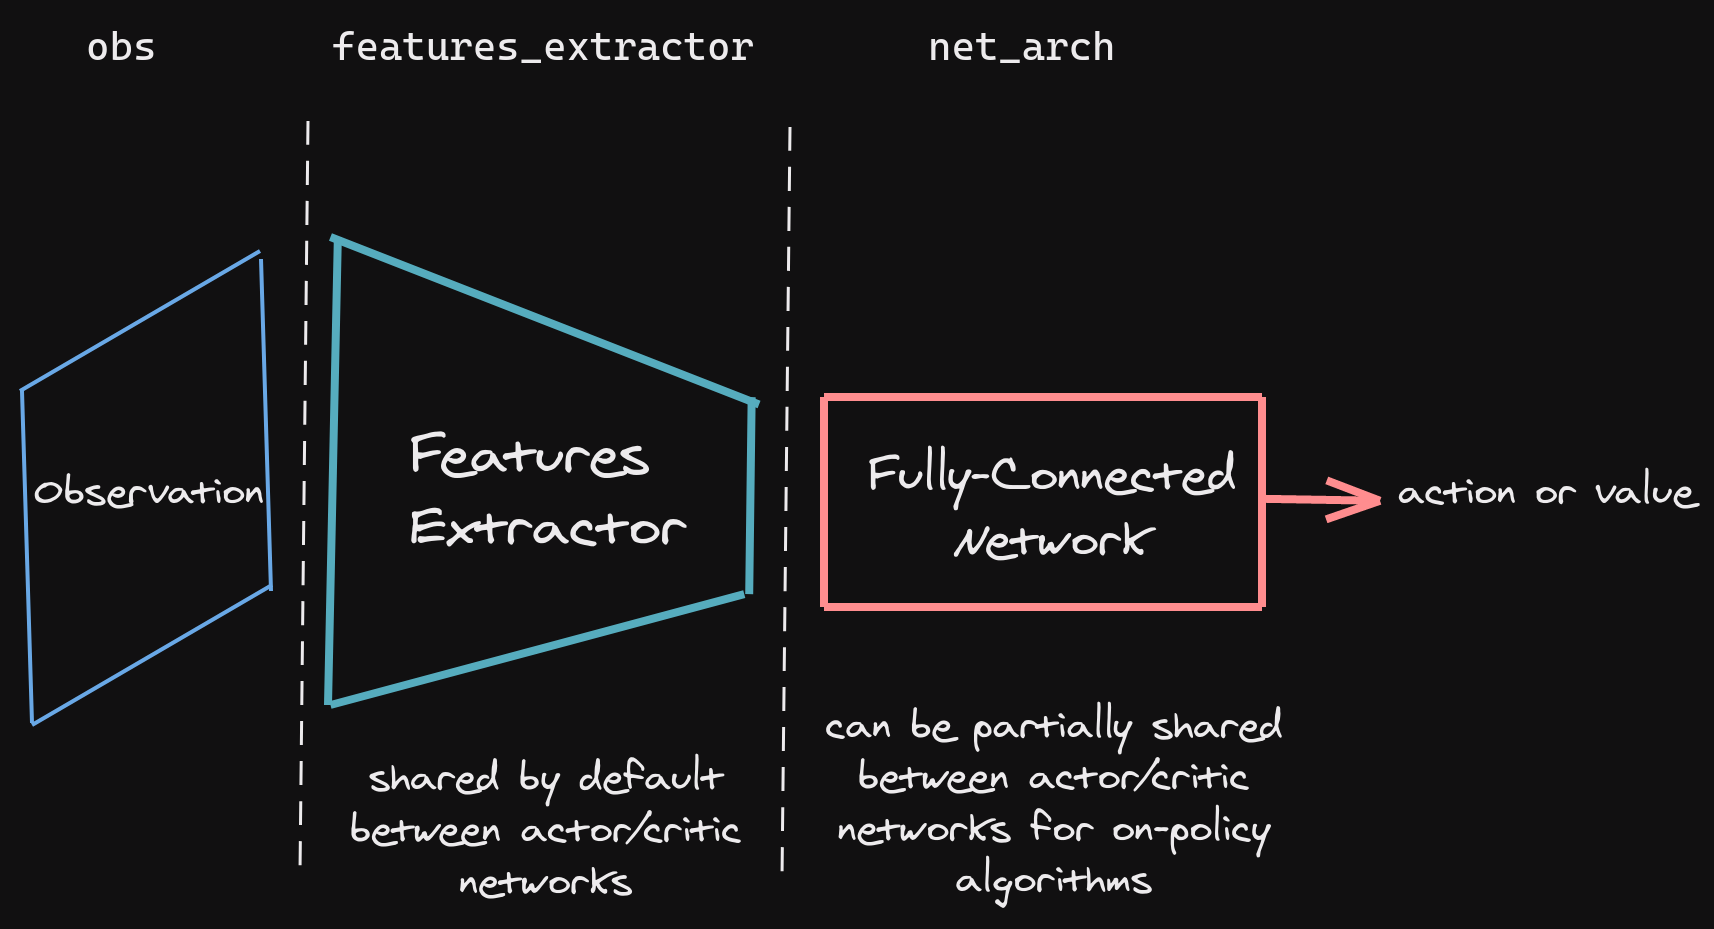
\includegraphics[width=0.65\textwidth]{pic/10}
    \caption{Архитектура CnnPolicy[24]}
    \label{fig:img1}
\end{figure}

В видеоиграх получать информацию о среде проще всего через скриншот того, что происходит на экране. Таким образом сотояния среды можно определять через эти скриншоты, поэтому 
в качестве агента была выбрана модель CnnPolicy, реализованная в библиотеке Stable Baselines3. Архитектура, данной модели, представляет из себя последовательный ансамбль
из двух алгоритмов: предобученной CNN, с помощью которой происходит извлечение признаков из входного изображения для получения текущего состояния среды, и RL алгоритма PPO, описанного
в теоретической части работы, в основе которого лежит архитектура Actor-critic. Архитектура CnnPolicy схематично изображена на рисунке 9.

В качестве функции потерь агента была использована функция кросс-энтропии, а в качестве функции потерь критика использовалась функция policy gradient.

\subsection{Процесс обучения агента}
Обучение агента выполнялось в Visual Studio Code на компьютере с установленной Windows 10 Pro с процессором AMD Ryzen 5 2600 графический процессор NVIDIA GeForce RTX 2070 SUPER.
Весь процесс последнего обучения в 560000 шагов с learning rate = 0.0001 и $\gamma$ = 0.95 проходил на GPU и занял примерно 3 часа 13 минут. Код для запуска обучения агента
находится в файле train.py.

В ходе обучения перед агентом стояла задача научится проходить данный сценарий с максимальной наградой. На превых шагах агент изучал окружающуюю его среду, путем выполнения
случайных действий. Таким образом на 100000 шаге он обучился определять, где находится первые враги и устранять их с минимальной потерей здоровья и патронов. Дальнейшей задачей
агента было понять, что для достижения своей цели ему нужно идти вперед, что было достинуто уже примерно на 200000 шаге. После чего агент учился совмещать два вышеописанных действия.
Эта цель была достигнута на 350000 шаге. Далее агент учился минимизировать урон, получаемый от врагов, путем стрельбы из-за стены, чтобы быть в радиусе видимости только одного
врага, что было тоже достигнуто спустя 80000 шагов. Последней задачей, которая осталась у агента было дохождение до брони и тем самым завершение игры, так как после устранения
всех препятствий на своем пути, он не понимал, что дальше делать, думая, что в конце тупик и возвращался в начало. Эта проблема была решена на 480000 шаге, когда агент впервые
завершил поставленную перед ним задачу. Последние свои шаги обучения агент старался, используя все, что уже выучил минимизировать свои потери, чтобы получить большую награду,
с чем успешно справился.

\subsection{Результаты обучения}
Значения функций потерь на момент окончания обучения представлены на рисунке 10. По ним видно, что основные функции потерь, по которым шла минимизация ошибки имеют очень маленькое
значение, что свидетельствует о хорошем обучении модели.

\begin{figure}[H]
    \centering
    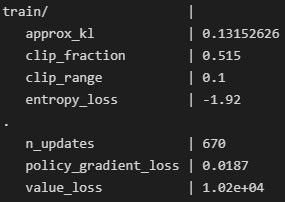
\includegraphics[width=0.45\textwidth]{pic/11}
    \caption{Вывод значений функций ошибки}
    \label{fig:img1}
\end{figure}

В качестве основной метрики была выбрана метрика ep_rew_mean - это значение средней награды за несколько эпизодов. В данном случае это средняя награда за 8192 шагов, что примерно
эквивалентно 100 эпизодам. Эта оценка является действительным числом в диапозоне от минимальной награды за эпизод до максимальной наград за эпизод и, чем оно больше, тем лучше.

\begin{figure}[H]
    \centering
    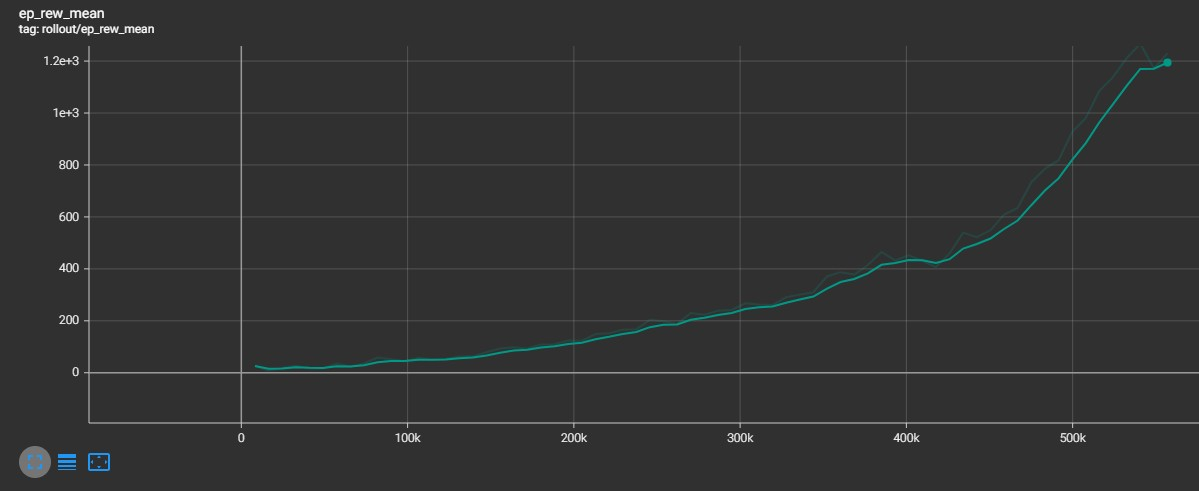
\includegraphics[width=0.85\textwidth]{pic/13}
    \caption{График кривой обучения, где на OX обозначены значения номер шага, а на оси OY - значения метрики ep_rew_mean}
    \label{fig:img1}
\end{figure}

При последней проверки качества модели были запущены 100 эпизодов, в результате которых значение метрики метрики ep_rew_mean было равно 1314.9392428588867, максимальная награда
за эпизод составила 3457.0574798583984, а минимальная - -1213.6784362792969. Код для проверки метрик и теста модели находится в файле test.py.
\newpage
\conclusion %заключение

В теоретической части данной работы были рассмотрены основные понятия, концепции и алгоритмы обучения с подкреплением, в связи с чем были так же рассмотрены такие темы как:
искусственный интелект, нейронный сети, обучение нейронных сетей и обучение с подкреплением в том числе, принцип работы сверточных нейронных сетей, а также понятие метрик моделей,
метрики, используемой в задачах обучения с подкреплением.

В практической части работы была описана реализация алгоритма, обучаемого с подкреплением для игры в DOOM, обучена модель и представлены результаты обучения в виде метрики модели,
значений функции потерь и кривых обучения.

\begin{thebibliography}{3}
    \bibitem{1}
    Пять технологий искусственного интелекта, о которых вам нужно знать [Электронный ресурс] – URL: https://www.sas.com/ru_ru/insights/articles/analytics/five-ai-technologies.html (дата обращения 27.04.2021) - Загл. с экрана. Яз. рус.
    \bibitem{2}
    Нейронные сети для начинающих. Часть 1 [Электронный ресурс] – URL: https://habr.com/ru/post/312450/ (дата обращения 13.05.2022) - Загл. с экрана. Яз. рус.
    \bibitem{3}
    А. Стариков "Нейронные сети — математический аппарат" [Статья] – URL: https://basegroup.ru/community/articles/math (дата обращения 13.05.2022) Яз. рус.
    \bibitem{4}
    Нейронные сети, или как обучить искусственный интеллект [Электронный ресурс] – URL: http://internetinside.ru/neyronnye-seti-ili-kak-obuchit-iskuss/ (дата обращения 13.05.2022) - Загл. с экрана. Яз. рус.
    \bibitem{5}
    Как работает нейронная сеть: алгоритмы, обучение, функции активации и потери [Электронный ресурс] – URL: https://neurohive.io/ru/osnovy-data-science/osnovy-nejronnyh-setej-algoritmy-obuchenie-funkcii-aktivacii-i-poteri/ (дата обращения 13.05.2022) - Загл. с экрана. Яз. рус.
    \bibitem{6}
    Сверточная нейронная сеть, часть 1: структура, топология, функции активации и обучающее множество [Электронный ресурс] – URL: https://habr.com/ru/post/348000/ (дата обращения 13.05.2022) - Загл. с экрана. Яз. рус.
    \bibitem{7}
    Обучение с подкреплением в машинном обучении [Электронный ресурс] – URL: https://evergreens.com.ua/ru/articles/reinforcement-learning.html (дата обращения 16.05.2022) - Загл. с экрана. Яз. рус.
    \bibitem{8}
    Как искусственный интеллект играет в «Змейку» [Электронный ресурс] – URL: https://habr.com/ru/company/skillfactory/blog/520992/ (дата обращения 16.05.2022) - Загл. с экрана. Яз. рус.
    \bibitem{9}
    Обучение с подкреплением [Электронный ресурс] – URL: https://neerc.ifmo.ru/wiki/index.php?title=Обучение_с_подкреплением (дата обращения 16.05.2022) - Загл. с экрана. Яз. рус.
    \bibitem{10}
    Интуитивная основа обучения с подкреплением [Электронный ресурс] – URL: https://nuancesprog.ru/p/13051/ (дата обращения 17.05.2022) - Загл. с экрана. Яз. рус.
    \bibitem{11}
    Катрина Уэйкфилд "Гид: алгоритмы машинного обучения и их типы" [Статья] – URL: https://www.sas.com/ru_ru/insights/articles/analytics/machine-learning-algorithms-guide.html (дата обращения 17.06.2022) - Загл. с экрана. Яз. рус.
    \bibitem{12}
    Обучение с подкреплением: разбираем на видеоиграх [Электронный ресурс] – URL: https://habr.com/ru/company/smileexpo/blog/428329/ (дата обращения 17.05.2022) - Загл. с экрана. Яз. рус.
    \bibitem{13}
    Обучение нейросети с учителем, без учителя, с подкреплением — в чем отличие? Какой алгоритм лучше? [Электронный ресурс] – URL: https://neurohive.io/ru/osnovy-data-science/obuchenie-s-uchitelem-bez-uchitelja-s-podkrepleniem/ (дата обращения 17.05.2022) - Загл. с экрана. Яз. рус.
    \bibitem{14}
    Deep Reinforcement Learning: как научить пауков ходить [Электронный ресурс] – URL: https://habr.com/ru/post/483078/ (дата обращения 17.05.2022) - Загл. с экрана. Яз. рус.
    \bibitem{15}
    Intro to Policy Optimization [Электронный ресурс] – URL: https://spinningup.openai.com/en/latest/spinningup/rl_intro3.html (дата обращения 17.05.2022) - Загл. с экрана. Яз. англ.
    \bibitem{16}
    L. Weng "Policy Gradient Algorithms" [Статья] – URL: https://lilianweng.github.io/posts/2018-04-08-policy-gradient/ (дата обращения 17.05.2022) - Загл. с экрана. Яз. англ.
    \bibitem{17}
    Е. Р. Чичадзе "Сравнительный анализ алгоритмов Proximal Policy Optimization И Soft-Actor-Critic" [Статья] – URL: https://cyberleninka.ru/article/n/sravnitelnyy-analiz-algoritmov-proximal-policy-optimization-i-soft-actor-critic/viewer (дата обращения 17.05.2022) Яз. рус.
    \bibitem{18}
    Учебное пособие по оптимизации проксимальных политик [Электронный ресурс] – URL: https://www.machinelearningmastery.ru/proximal-policy-optimization-tutorial-part-1-actor-critic-method-d53f9afffbf6/ (дата обращения 17.05.2022) - Загл. с экрана. Яз. рус.
    \bibitem{19}
    Что не так с обучением с подкреплением (Reinforcement Learning)? [Электронный ресурс] – URL: https://habr.com/ru/post/437020/ (дата обращения 17.05.2022) - Загл. с экрана. Яз. рус.
    \bibitem{20}
    Reinforcement Learning (DQN) tutorial [Электронный ресурс] – URL: https://pytorch.org/tutorials/intermediate/reinforcement_q_learning.html (дата обращения 17.05.2022) - Загл. с экрана. Яз. англ.
    \bibitem{21}
    OpenAI Five [Электронный ресурс] – URL: https://openai.com/five/ (дата обращения 21.05.2022) - Загл. с экрана. Яз. англ.
    \bibitem{22}
    D. Biswas "Self-improving Chatbots based on Deep Reinforcement Learning" [Статья] – URL: https://towardsdatascience.com/self-improving-chatbots-based-on-reinforcement-learning-75cca62debce (дата обращения 21.05.2022) - Загл. с экрана. Яз. англ.
    \bibitem{23}
    M. Berk "How to Use Reinforcement Learning to Recommend Content" [Статья] – URL: https://towardsdatascience.com/how-to-use-reinforcement-learning-to-recommend-content-6d7f9171b956 (дата обращения 21.05.2022) - Загл. с экрана. Яз. англ.
    \bibitem{24}
    Документация Stable Baselines3 [Электронный ресурс] – URL: https://sb3-contrib.readthedocs.io/en/master/index.html (дата обращения 21.05.2022) Яз. англ.
    \bibitem{25}
    Документация PyTorch [Электронный ресурс] – URL: https://pytorch.org/ (дата обращения 21.05.2022) Яз. англ.
    \bibitem{26}
    Документация OpenCV [Электронный ресурс] – URL: https://docs.opencv.org/4.x/d6/d00/tutorial_py_root.html (дата обращения 21.05.2022) Яз. англ.
    \bibitem{27}
    Документация OpenAI Gym [Электронный ресурс] – URL: https://www.gymlibrary.ml/ (дата обращения 21.05.2022) Яз. англ.
    \bibitem{28}
    Репозиторий на GitHub со сценариями DOOM [Электронный ресурс] – URL: https://github.com/mwydmuch/ViZDoom (дата обращения 21.05.2022) Яз. англ.
\end{thebibliography}

\appendix

    \section{Код environment.py}
    \inputminted[fontsize=\footnotesize]{text}{../environment.py}

    \section{Код train.py}
    \inputminted[fontsize=\footnotesize]{text}{../trainer.py}

    \section{Код test.py}
    \inputminted[fontsize=\footnotesize]{text}{../test.py}

\end{document}